\documentclass[14pt]{beamer}

\usepackage[british]{babel}

\usepackage{graphicx}
\usepackage{amssymb}
\usepackage{color}

\usepackage{listings}
\usepackage{prettylistings}
\usepackage{lang-llvm}
\usepackage{lang-spl}
\usepackage{lang-ssm}

\usepackage{xspace}
\usepackage{url}

\usepackage{array}

\newcommand{\splang}{\textsc{Splang}\xspace}
\newcommand{\llvm}{\textsc{LLVM}\xspace}
\newcommand{\demo}{\raisebox{0.2cm}{\tiny[\textsc{Demo}]}\xspace}

\newcommand{\SPL}{\texttt{SPL}\xspace}
\newcommand{\C}{\texttt{C}\xspace}
\newcommand{\Cpp}{\texttt{C}$^{++}$\xspace}

\newcommand{\spl}[1]{\lstinline[language=spl,basicstyle=]{#1}}

\title{\splang}
\author{Wouter Geraedts \and Joshua Moerman}
\institute{Radboud Universiteit Nijmegen}
\date{}

\begin{document}

\begin{frame}
	\titlepage
\end{frame}

\begin{frame}
	\frametitle{\llvm}

	\begin{itemize}
		% LLVM used to stand for low level virtual machine, but as it also is capable of native codegen, they dropped the acronym
		\item \emph{Low Level Virtual Machine}\footnote{Not only a VM, but also native codegen!}
		\item We generate \llvm IR:
		\begin{itemize}
			\item Strongly typed (no polymorhpism)
			\item Single assignment
		\end{itemize}
	\end{itemize}

	\bigskip
	\pause
	\begin{center}
		Why?
	\end{center}
\end{frame}

\begin{frame}
\begin{center}
	\frametitle{What we get for ``free''}
	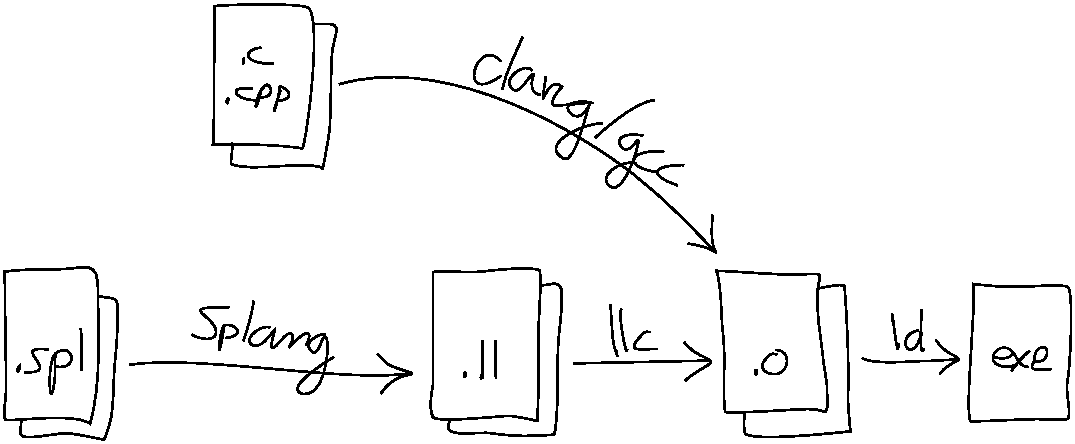
\includegraphics[width=\textwidth]{linking}
	\bigskip

	Native codegen, \quad Optimizations,\\
	Linking with \C, \Cpp, \quad JIT
\end{center}
\end{frame}

\begin{frame}
	\frametitle{Bindings}
	There are Haskell bindings for \llvm (via a \C API), but we couldn't get it to work.

	\bigskip
	So we have to output the IR ourself!
\end{frame}

\begin{frame}
	\frametitle{Example (Strongly typed)}
	\lstinputlisting[language=llvm]{llvm-struct.ll}
\end{frame}

\begin{frame}
	\frametitle{Example (Single assignment)}
	\lstinputlisting[language=llvm]{llvm-alloca.ll}
\end{frame}

\begin{frame}
	\frametitle{Linking with \C}
	Added \spl{extern "lang"} to the syntax:
	\lstinputlisting[language=spl]{spl-externc.spl}

	\pause
	Also works with \spl{extern "SPL"} (seperate compilation)!
\end{frame}

\begin{frame}
\begin{center}
	{\Huge Demo!}

	calling \C from \SPL

	calling \SPL from \SPL
\end{center}
\end{frame}

\begin{frame}
	\frametitle{Templating}
	Recall that we do \emph{templating}. I.e.: only generate what is needed.

	\bigskip\pause
	But what is needed? Everything reachable from main?

	\bigskip\pause
	Breaks seperate compilation...

	Added \spl{export} to the syntax:
	\lstinputlisting[language=spl]{spl-export.spl}
\end{frame}

\begin{frame}
\begin{center}
	{\Huge Demo!}

	calling \SPL from \Cpp

	JIT
\end{center}
\end{frame}

\begin{frame}
\begin{center}
	{\Huge Demo!}

	calling \SPL from \Cpp

	JIT
\end{center}
\end{frame}

\begin{frame}
\begin{center}
	\frametitle{Fun: all our phases :)}
	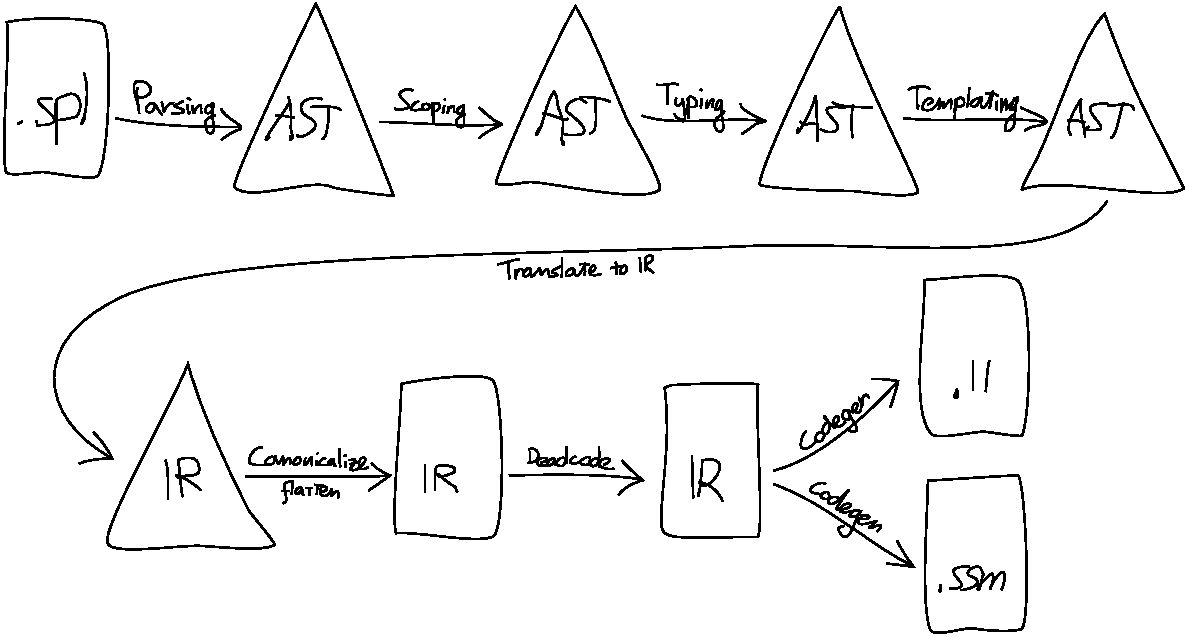
\includegraphics[width=\textwidth]{phases}
\end{center}
\end{frame}

\end{document}
